\section{Ising model}

\subsection{Ising model in statistical mechanics}

\begin{frame}{Phase Transitions}
	\begin{columns}
		\begin{column}{0.5\textwidth}
			A major topic of interest in statistical mechanics (and in physics in general) is the understanding of \alert{phase transitions} (e.g. freezing of water to form ice), which requires the study of \alert{interacting models}.
		\end{column}
		
		\begin{column}{0.5\textwidth}
			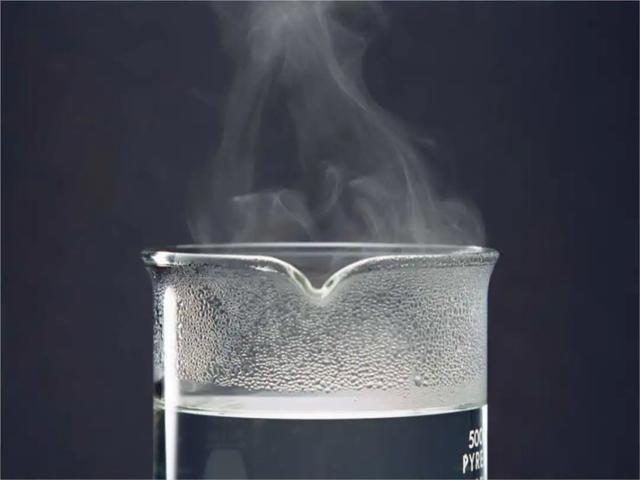
\includegraphics[width = 0.9\textwidth]{Figures/phase.jpeg}
			\centerline{water $\longrightarrow$ vapour}
		\end{column}
	\end{columns}
\end{frame}

\begin{frame}{Ferromagnetic phase transition}
	\begin{columns}
		\begin{column}{0.5\textwidth}
			\centerline{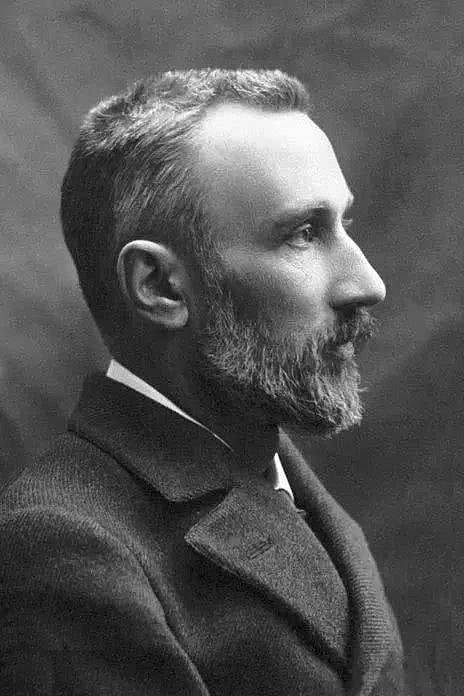
\includegraphics[width = 0.6\textwidth]{Figures/pi.jpg}}
			\centerline{Pierre Curie (1895)}
		\end{column}
		
		\begin{column}{0.5\textwidth}
			\centerline{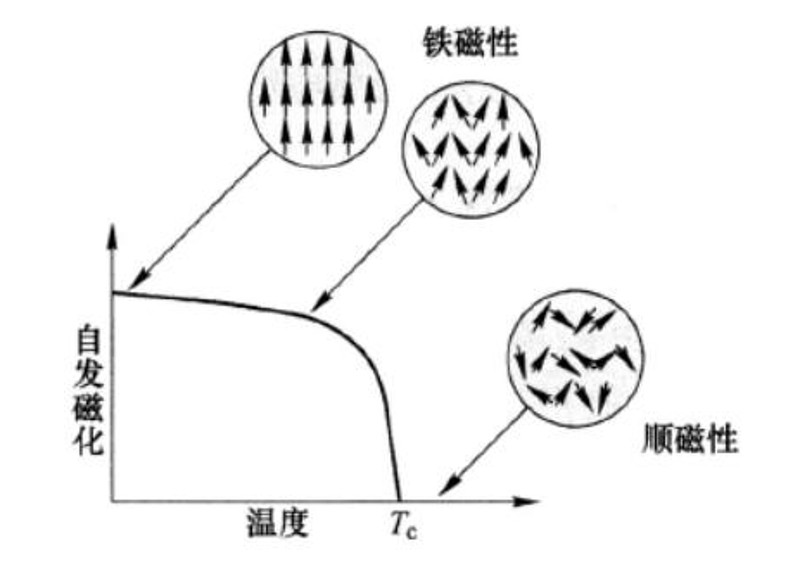
\includegraphics[width = 1.0\textwidth]{Figures/tr.jpg}}
			Why does the magnetism lose after heating the magnet beyond a certain temperature?
		\end{column}
	\end{columns}
	
\end{frame}

\begin{frame}{Background}
	\begin{columns}
		\begin{column}{0.5\textwidth}
			\centerline{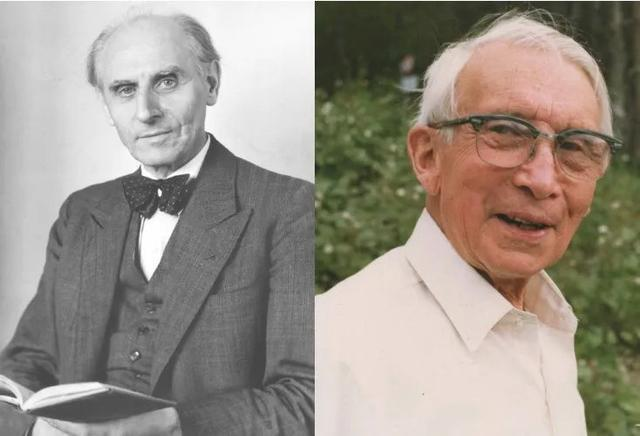
\includegraphics[width = 0.9\textwidth]{Figures/teacher.jpeg}}
			\centerline{Wilhelm Lenz and Ernst Ising}
			\centerline{(Teacher-student relationship)}
		\end{column}
		
		\begin{column}{0.5\textwidth}
			The Main ideas:
			\begin{itemize}
				\item Lenz considered the inside of the matter as a grid, where each node contains an atom represented by \alert{a simplified arrow}.
				\item Ising applied \alert{the principle of the lowest energy}. The magnetic forces tend to keep neighbouring arrow in the same direction, while disturbances will destroy this tendency.
			\end{itemize}
		\end{column}
	\end{columns}
\end{frame}

\begin{frame}{Definition of Ising model}
	\cite[pp.~74--75]{Ising model (1925)}
	\begin{definition}
		\begin{enumerate}
			\item A periodic lattice;
			\item With “spin” variables $s_i$, which can only take the values +1 (↑) and -1 (↓);
			\item Every spin interacts with its nearest neighbors as well as with an external magnetic field $h$.
		\end{enumerate}
		
	\end{definition}
	The Hamiltonian (system energy) of the Ising model is
	$$H\left(\left\{s_{i}\right\}\right)=-J \sum_{\langle i, j\rangle} s_{i} s_{j}-h \sum_{i} s_{i}$$
	The sum $<i,j>$ is over nearest neighbors. $J$ is a constant specifying the strength of interaction. 
\end{frame}

\begin{frame}{Schemic}
\begin{columns}
	\begin{column}{0.5\textwidth}
		\centerline{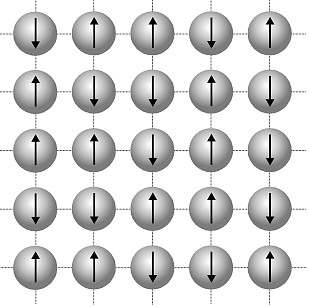
\includegraphics[width = 0.9\textwidth]{Figures/2d.jpg}}
		\centerline{Ising model in 2D}
	\end{column}
	
	\begin{column}{0.5\textwidth}
		It can be used to describe many physical phenomena, such as
		\begin{itemize}
			\item the order-disorder transition in alloys
			\item the transition from liquid helium to superfluid
			\item the freezing and evaporation of liquids
			\item the properties of glass substances
			\item forest fires
			\item urban traffic......
		\end{itemize}
	\end{column}
\end{columns}
	\end{frame}

\begin{frame}{Statistical Mechanics}
	The Ising model is usually studied in \alert{the canonical ensemble}. (It would be a nightmare to do it in the microcanonical ensemble.)
\begin{theorem}
	In the canonical ensemble, the probability of finding a particular spin configuration $\left\{s_{i}\right\}$ is,
	$$p\left(\left\{s_{i}\right\}\right)=\frac{1}{Z} \exp \left(-\beta H\left(\left\{s_{i}\right\}\right)\right), \quad \beta \equiv \frac{1}{k_{B} T}$$
	where $Z=\sum_{\left\{s_{i}\right\}} \exp \left(-\beta H\left(\left\{s_{i}\right\}\right)\right)$ is the partition function. 
\end{theorem}

Due to the Boltzmann factor, $\mathrm{e}^{-\beta H}$, spin configurations with lower energies will be favored.
\end{frame}

\begin{frame}{Two parameters}
	We can now discuss the effect of $J$ and $h$ on the behavior of the spins.
	\begin{itemize}
		\item when $h > 0$, $si = +1$ is favored.
		\item when $h < 0$, $si = -1$ is favored.
	\end{itemize}
	This means that the spins wants to align with the direction of $h$.
	\begin{itemize}
		\item when $J > 0$, neighboring spins prefer to be parallel. (This is called the ferromagnetic model.)
		\item when $J < 0$, neighboring spins prefer to be anti-parallel. (This is called the anti-ferromagnetic model.)
	\end{itemize}
	
\end{frame}

\begin{frame}{Explanation of the transition}
	\cite[pp.~74--75]{At low enough temperature:}
	\begin{description}
		\item[Spontaneous magnetization] All spins in the Ising model will spontaneously align themselves even in the absence of the external field ($h = 0$).
	\end{description}
	
	\cite[pp.~74--75]{At high enough temperature:}
	\begin{itemize}
		\item The spontaneous magnetization is destroyed by thermal fluctuation.
		\item There is a critical temperature $T_c$, below which there is spontaneous magnetization and above which there isn’t.
		\item There is a phase transition at $T_c$.
	\end{itemize}
	
\end{frame}

\begin{frame}{Traditional Implementations}
	\begin{table}[ht]
		\centering
		\begin{tabular}{c || c || c || c}
	\textbf{\begin{CJK}{UTF8}{gkai}文件数目
	\end{CJK}} &\begin{CJK}{UTF8}{gkai}Worker数目
\end{CJK} &\textbf{\begin{CJK}{UTF8}{gkai}串行耗时
\end{CJK}} &\textbf{\begin{CJK}{UTF8}{gkai}并行耗时
\end{CJK}}\\
	\hline
	50 &4 &9.4s &31s\\
	\hline
	100 &4 &19.9s &56.23s\\
	\hline
	150 &4 &32s &83s\\
	\hline
	200 &4 &38.8s &106.2s\\
	
	
\end{tabular}

		%\caption{Table 1}
	\end{table}
	\centerline{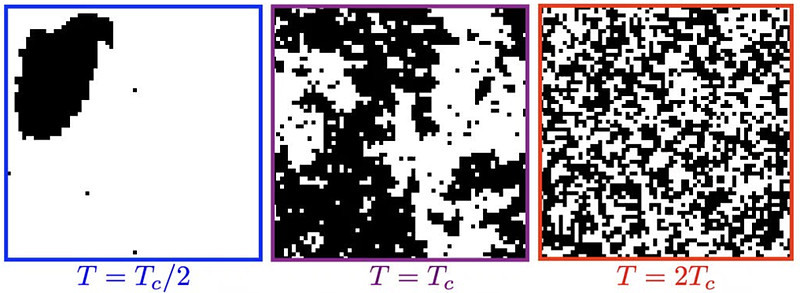
\includegraphics[width = 0.7\textwidth]{Figures/im.jpg}}
\end{frame}
